\documentclass[12pt]{article}
\usepackage[]{graphicx}
\usepackage[]{color}
\usepackage{amsmath, amsfonts, amssymb, amsthm, latexsym}
\usepackage{multicol}
\usepackage{graphicx}
\usepackage{longtable}
\usepackage{titlesec}

\usepackage[margin=2.4cm]{geometry}
\setlength{\parindent}{0cm}

\setcounter{secnumdepth}{4}

\titleformat{\paragraph}
{\normalfont\normalsize\bfseries}{\theparagraph}{1em}{}
\titlespacing*{\paragraph}
{0pt}{3.25ex plus 1ex minus .2ex}{1.5ex plus .2ex}

\providecommand{\ds}{\displaystyle}
\providecommand{\abs}[1]{\left\vert#1\right\vert}
\newcommand{\given}{\hspace{3pt}|\hspace{3pt}}
\newcommand{\blip}{\hspace{2pt}}

\begin{document}
{\Large {\bf Summary}}\\
This report describes population model analyses done in support of the evaluation of management actions for pallid sturgeon on the Upper Missouri River, from Fort Peck Dam to Lake Sakakawea, using a population projection matrix.  The particular management actions of focus were alternative flow release protocols from Fort Peck Dam.  Seven alternative scenarios were considered:  No action, Alternative 1, Alternative 1a, Alternative 1b, Alternative 2, Alternative 2a, and Alternative 2b.  Additionally, potential effects of temperature and turbidity manipulations are explored.   Alternative scenarios were compared in terms of their ability to be fully implemented throughout the period of record, maximum discharge, estimated effects on drifting free-embryo retention, and predicted long-term growth rate.  Sensitivity and elasticity analyses were also conducted to demonstrate the effects of parameter values, including uncertainties in age-0 survival and probability of spawning in the Missouri River, on long-term population growth rate.  Limitations and uncertainties in the modeling, including caveats on the use of these models to estimate historical conditions and the availability of information to build a population model, are discussed.  Important future directions for the population model, such as incorporating fish passage at Intake in the Yellowstone, are also introduced.  

\begin{section}{Introduction}
\end{section}

\begin{section}{Methods}
\begin{subsection}{Modeling Framework \& Spatial Extent}
Seven alternative management scenarios at Fort Peck Dam were considered.   Details of the management scenarios:  No action, Alternative 1, Alternative 1a, Alternative 1b, Alternative 2, Alternative 2a, and Alternative 2b, are described in \textit{REFERENCE HERE}.  For each alternative, long-term population growth rate ($\lambda$) was estimated for the population of pallid sturgeon residing within the Upper Missouri River from Fort Peck Dam to Garrison Dam, including the Yellowstone River up to the Intake Diversion Dam (Figure 1).  The modeling framework used to calculate long-term population growth relied upon several submodels, including hydrological models, a spawning probability model, a drift-dispersion model, a free-embryo development model, and a pallid sturgeon demographic population model (Figure 2).  

\begin{subsubsection}{Hydrology, Drift, Development, \& Probability of Retention}
%Hydrological data were generated using the Hydrologic Engineering Centers Reservoir Simulation (HEC-ResSim) software implemented for the Missouri River reach between Fort Peck Dam and Lake Sakakawea. HEC-ResSim uses historical basin runoff data and specified rule sets defining reservoir operations to project reservoir inflows, outflows, and pool elevations as well as flows at additional points along the river. All hydrological runs used for this analysis used historical runoff from the period of record of 1930--2015. Reservoir operations were modeled for each alternative scenario assuming the same operation rules were in effect for all years.   Metrics (what are these, temporal and spatial scales) were calculated from daily ResSim output for use in the spawning and free-embryo drift-dispersion models.  The probability of free-embryo retention within the free-flowing Missouri River was computed by integrating a free-embryo developement model into HEC-RAS simulations, assuming spawning occurs just below Fort Peck dam.
Hydrological data were generated using the Hydrologic Engineering Centers Reservoir Simulation (HEC-ResSim) software implemented for the Missouri River reach between Fort Peck Dam and Lake Sakakawea (see \textit{REFERENCE} for further HEC-ResSim modeling details).  All hydrological runs used for this analysis used historical runoff from the period of record of 1930--\textit{2017}.  Reservoir operations were modeled for each alternative scenario assuming the same operation rules were in effect for all years.   For each scenario and year on record, HEC-ResSim outputs were used to compute the probability a reproductively-ready female spawns in the Missouri River (rather than spawning in the Yellowstone River or reabsorbing her eggs) and the probability that a free-embryo develops to settlement prior to reaching the unfavorable conditions of Lake Sakakawea (retention probability). The probability of free-embryo retention within the free-flowing Missouri River was computed by integrating a temperature dependent free-embryo development model into HEC-RAS drift simulations, assuming spawning occurs just below Fort Peck dam.  The details of this modeling are described in \textit{REFERENCE HERE}.  
\end{subsubsection}

\begin{subsubsection}{Hydrology and Spawning Probability}
The factors effecting the probability a reproductively-ready female spawns within the Missouri River are largely uncertain.  Limited data has shown \textit{FILL IN THIS SECTION}.\\
 
As a first approach, the probability a reproductively-ready female spawns in the Missouri River ($\gamma$) was modeled in terms of discharge and temperature as a multi-variate step function:
\begin{equation}
\gamma(Q, T) = \begin{cases}
\gamma_{high}, & \hspace{0.5cm}  Q\geq Q^{*} \hspace{12pt} \& \hspace{12pt} T\geq T^{*}\\
%\gamma_{med}, & \hspace{0.5cm}  Q\geq Q^{*} \& T_{sp, low} \leq T< T^{*}\\
\gamma_{low}, & \hspace{0.5cm}  Q< Q^{*} \hspace{12pt} \mbox{or} \hspace{12pt} T< T^{*}
\end{cases},
\end{equation}
where\\

\hspace*{0.5cm}$Q$ is the \textit{maximum} discharge \textit{during April--May} in cfs,\\
\hspace*{0.5cm}$Q^{*}$ is the threshold discharge needed to attract and retain spawners up the Missouri River\\ 
\hspace*{1.5cm}to the vicinity of Fort Peck Dam (in cfs),\\
\hspace*{0.5cm}$T$ is the maximum temperature reached below Fort Peck Dam during \textit{the end of May--\\
\hspace*{1.5cm}beginning of July} in $^{\circ}$C,\\
\hspace*{0.5cm}$T^{*}$ is the threshold temperature required for spawning (in $^{\circ}$C),\\
\hspace*{0.5cm}$\gamma_{high}$ is the probability that a reproductively-ready female will spawn in the Missouri River\\ 
\hspace*{1.5cm}below Fort Peck Dam given favorable flow and temperature conditions, and\\
\hspace*{0.5cm}$\gamma_{low}$ is the probability that a reproductively-ready female will spawn in the Missouri River\\
\hspace*{1.5cm}below Fort Peck Dam given unfavorable conditions.\\

Baseline values for $Q^{*}$, $T^{*}$, $\gamma_{high}$, and $\gamma_{low}$ were based on observed cases of female spawning migrations up the Missouri River above the confluence with the Yellowstone (Table 1).  Outputs from HEC-ResSim provide values for $Q$ and $T$, allowing $\gamma$ to be computed for each alternative scenario under any given year on record.   
\end{subsubsection} 

\begin{subsubsection}{Demographic Population Model}
The demographic pallid sturgeon population model is a prebreeding Leslie matrix model:
\begin{eqnarray}
N_{t+1} & = & AN_{t},\\
A & = &  \begin{pmatrix}
F_1 & F_2 & F_3 & \cdots & F_{a_{max}-1} & F_{a_{max}}\\
\phi_1 & 0 & 0 & \cdots  & 0 & 0\\
0 & \phi_2 & 0 & \cdots  & 0 & 0\\
0 & 0 & \phi_3 & \ddots & 0 & 0\\
\vdots & \vdots & \ddots  & \ddots & \vdots & \vdots\\
0 & 0 & 0 & \cdots & \phi_{a_{max}-1} & 0\\
\end{pmatrix},
\end{eqnarray}
where\\
\hspace*{0.5cm}$N_t$ is a vector of population sizes by age-class in year $t$,\\
\hspace*{0.5cm}$A$ is a Leslie matrix,\\
\hspace*{0.5cm}$F_i$ is the expected fertility value of an age-$i$ female pallid sturgeon,\\
\hspace*{0.5cm}$\phi_i$ is the probability that a female survives from age-$i$ to age-$i+1$, and\\
\hspace*{0.5cm}$a_{max}$ is the maximum age of a female fish.\\

The age-specific fertility values are functions of the probability of free-embryo retention ($p_{ret}$) and the probability a reproductively-ready female spawns in the Missouri River ($\gamma$) and vary by management alternatives (Figure 2).  Details of the model parameterization are described in the following three sections with baseline parameter values listed in Table 1.\\

\paragraph{Maximum Age}
The baseline maximum age of a female pallid sturgeon was taken to be 60 years old.  Bratten et al. (2015) estimated the ages of 11 deceased natural-origin pallid sturgeon from the Upper Missouri River.  They determined longevity to be at least 50 years, with individual estimates ranging from 37-59 years old.\\

\paragraph{Age-Specific Survivals}
Age-specific survivals were estimated for pallid sturgeon ages 1 through 9 years old utilizing data from Rotella et al.'s Upper Basin Pallid Sturgeon Survival Estimation Project 2017 Update.  Only data for fingerlings released in RPMA 2 in the Missouri River with an ``IV status'' and ``fin curl status'' of zero were analyzed.  Fingerlings, released into the river at about 3 months old, were chosen with the expectation that having 9 months to acclimate to river conditions would allow for a better estimate of natural age-1 to age-2 survival than yearlings released into the river much closer to their first birthday.  For each cohort meeting the specified criteria, population estimates across each interval time period available were used to calculate daily survival as
\begin{equation}
\mbox{Interval Daily Survial}=\left(\frac{N \mbox{ at Interval End}}{N \mbox{ at Interval Start}}\right)^{1/\mbox{{\scriptsize Days in Interval}}}.
\end{equation}

Cohort-specific interval daily survivals were then used to compute cohort-specific survivals from age-class to age-class, assuming all fish were born on June 1st.  The weighted average of cohort-specific annual survivals was used as an estimated for the age-specific annual survivals:
\begin{equation}
\phi_i=\frac{\displaystyle\sum_{c \hspace{1pt} \in \hspace{1pt} C} \phi_{i,c}N_{i,c}}{\displaystyle\sum_{c \hspace{1pt} \in \hspace{1pt} C} N_{i,c}},
\end{equation} 
where\\
\hspace*{0.5cm}$\phi_i$ is the age-$i$ survival probability for ages $i=1, 2, \ldots, 9$,\\
\hspace*{0.5cm}$\phi_{i,c}$ is the probability that a fish in cohort $c$ survives from age-$i$ to age-$i+1$,\\ 
\hspace*{0.5cm}$N_{i,c}$ is the expected number of age-$i$ fish in cohort $c$ on June 1st, and\\
\hspace*{0.5cm}$C$ is the set of all healthy cohorts (IV=0, Fin Curl=0) released into the Missouri River\\ 
\hspace*{1.5cm}within RPMA 2 as fingerlings.\\

Adult annual survival ($\phi_{adult}$) was computed from RPMA 2 wild adult population estimates in 2004 and 2008 (Klungle \& Baxter 2004, Jaeger et al. 2008) as
\begin{equation}
\phi_{adult}=\left(\frac{125}{158}\right)^{1/4}\approx 0.94,
\end{equation}
and set as the survival probability of all females age-15 and older.  Survival probabilities for age-10 to age-14 pallid sturgeon were extrapolated ad hoc from the probabilities computed for younger and older fish (Figure 3, Table 1).\\

  



\paragraph{Age-Specific Fertilities}
Age-specific fertility values ($F_i$) were broken down into several components:
\begin{equation}
F_i=\psi_i\gamma E_ir\phi_{0}p_{ret},
\end{equation}
where\\
\hspace*{0.5cm}$\psi_i$ is the proportion of age-$i$ females that are reproductively ready to spawn,\\
\hspace*{0.5cm}$\gamma$ is the fraction of reproductively ready females that spawn in the Missouri River,\\
\hspace*{0.5cm}$E_i$ is the number of eggs per spawning age-$i$ female,\\ 
\hspace*{0.5cm}$r$ is the sex ratio (fraction of the eggs that are female),\\
\hspace*{0.5cm}$\phi_{0}$ is the survival from egg to age-1 given retention within the free-flowing Missouri\\
\hspace*{1.5cm}River, and\\
\hspace*{0.5cm}$p_{ret}$ is the probability a drifting free-embryo is retained in the free-flowing Missouri River.\\

Only age-0 survival is considered for those fish retained in the free-flowing Missouri River ($\phi_{0}$) because it is assumed that survival in the anoxic conditions of Lake Sakakawea is zero.   For the baseline analysis estimating current conditions, it is assumed that retention probability is 1 in 1,000 and spawning in the Missouri River occurs about once every 100 years (Table 1).   In general, both the retention probability ($p_{ret}$) and the probability a reproductively-ready female spawns within the Missouri River ($\gamma$) are assumed to be directly effected by temperature and flow.  Therefore, they vary with environmental conditions, as well as choice of management action.   For the Fort Peck Flows analyses, $p_{ret}$ and $\gamma$ are estimated as outputs of the drift-development and spawning models, respectively, given the particular management alternative scenario and hydrology.  The remaining parameter values ($r$, $\phi_0$, $\psi_i$, and $E_i$) are fixed among scenarios, and described in detail below.\\ 

\textbf{\underline{Sex Ratio and Age-0 Survival}}\\

\vspace{-6pt}Both the probability a fish is female ($r$) and the probability of surviving from egg to age-1 given retention in the Missouri River ($\phi_0$) are constants, independent of the mother's age.  The baseline sex ratio $r$ was computed from a 2008 Upper River (RPMA 2) estimate of 125 wild adults and 40 wild female adults (Jaeger et al. 2008), as
\begin{equation}
r=\frac{40}{125}= 0.32.
\end{equation} 
Missouri River age-0 survival is highly uncertain.  We set baseline Missouri River age-0 survival at an arbitrary, small probability of 75 in 1,000,000 or
\begin{equation}
\phi_0=0.000075.
\end{equation}
We further examine the sensitivity and robustness of model outcomes to changes in $\phi_0$.   Additionally, Missouri River age-0 survival likely varies with turbidity, and is an area of future consideration for linking management actions to population outcomes.\\

The probability a female is reproductively ready to spawn ($\psi_i$) and the expected number of eggs released per spawning female ($E_i$) are age-specific quantities.  Their baseline values were determined using multiple steps, as described first for $\psi_i$ and then for $E_i$ below.\\ 

\textbf{\underline{Probability a Female is Reproductively Ready ($\psi_i$)}}\\

\vspace{-6pt}The proportion of age-$i$ females that are reproductively ready is a function of maturation and spawning period:
\begin{equation}
\psi_i = \begin{cases}
m_i, & \hspace{1cm} i=0, 1, \ldots, a_m,\\
m_i + \sum_{j=a_{m}}^{i-1}\psi_{j}p_{i-j},  & \hspace{1cm} i=a_m+1, \ldots, a_{max}\\
\end{cases},
\label{psii}
\end{equation}
with
\begin{equation}
\sum_{i=1}^{a_{max}} m_i=1 \hspace{24pt} \mbox{ and } \hspace{24pt} \sum_{t=1}^{\infty} p_t =1,
\end{equation}
where\\ 
\hspace*{0.5cm}$\psi_i$ is the proportion of age-$i$ females that are reproductively ready to spawn,\\
\hspace*{0.5cm}$m_i$ is the proportion of age-$i$ females that just matured, i.e., the probability that the first\\ 
\hspace*{1.5cm}time a female is reproductively ready to spawn is when she is age-$i$,\\
\hspace*{0.5cm}$p_t$  is the probability that the period of time between being reproductively ready is $t$ years,\\
\hspace*{0.5cm}$a_m$ is the minimum age at which a female matures, and\\
\hspace*{0.5cm}$a_{max}$ is the maximum age of a female fish.\\


The maturation age of female pallid sturgeon has not been well studied and is an area of further informational need (Delonay et al. 2016).  Age of maturation could also vary by region of the river (George et al. 2012) with observations from the Upper Missouri River suggesting that female pallid sturgeon mature much later than those in the Lower Missouri and Mississippi Rivers (Molly Webb, personal communication).  What published data is available, involves only a handful of fish that are primarily from the Lower Missouri and Mississippi Rivers.   These females were estimated to have matured between the ages of 8 and 20 years old (Keenlyne \& Jenkins 1993, George et al. 2012).  Aging of the fish was typically performed by pectoral fin ray analysis, a method that can suffer from low accuracy and precision (Hurley et  al. 2004). 


We used a logistic cumulative distribution model to roughly describe maturation of females as they age:
\begin{equation}
F(a)=\frac{1}{1+e^{-k(a-a_h)}}
\label{cdf}
\end{equation}  
where\\
\hspace*{0.5cm}$F(a)$ is the proportion of age-$a$ females that have reached maturity,\\
\hspace*{0.5cm}$a_h$ is the age at which half of all females are mature,\\ 
\hspace*{0.5cm}$k$ is a scaling parameter that controls the variance of the distribution, and\\
\hspace*{0.5cm}$a$ is age.\\

To account for later maturation ages in Upper River females, we assumed that 50\% of female pallid sturgeon reach maturity by age 15 ($a_h=15$), 5 years later than the expected value used by Wildhaber et al. (2017) for female's in the Lower Missouri River.  We also assumed $k=1$ (corresponding to approximately 5 years representing 3 standard deviations).  We converted this unbounded, continuous cumulative maturation distribution to a discrete probability distribution bounded between the ages of 8 and 21 (Figure 4), as follows: 
\begin{equation}
m_i = \begin{cases}
0, & \hspace{1cm} i=1, 2, \dots, a_m-1\\
F(i), & \hspace{1cm} i=a_m\\
F(i)-F(i-1), & \hspace{1cm} i=a_m+1, a_m+2, \ldots, a_M-1\\
1-F(i-1), & \hspace{1cm} a=a_M\\
0, & \hspace{1cm} i=a_M+1, a_M+2, \ldots, a_{max}
\end{cases},
\label{mi}
\end{equation} 
where\\
\hspace*{0.5cm}$a_m$ is the minimum age at which a female matures,\\
\hspace*{0.5cm}$a_M$ is the maximum age at which a female matures, and\\ 
\hspace*{0.5cm}$F$ is the cumulative distribution described in (\ref{cdf}).\\ 


The spawning period of female pallid sturgeon is likely 2-5 years (Delonay et al. 2016), although it has been estimated to be as great as 10 years in past studies using spawning bands (Dryer \& Sandvol 1993, Keenlyne \& Jenkins 1993).  Fuller et al. (2007) and DeLonay et al. (2016) assessed the reproductive readiness of a combined total of  28 female pallid sturgeon.  Their combined data shows that all 28 females had a reproductive period greater than 1 year ($p_1=0$).  Additionally, 8 females had a confirmed spawning period of 2 years with 13 others confirmed as having a spawning period greater than 2 years ($p_2=8/21$).  Of the 13 females whose spawning period was greater than 2 years, only the fates of 5 were known beyond this point: 3 females had a confirmed spawning period of 3 years and 2 females had a confirmed spawning period that was greater than 3 years ($p_3=(13/21)(3/5)$).  Under the following additional assumptions:
\begin{enumerate}
\item the maximum reproductively ready period of a female is 5 years, and
\item a female is approximately twice as likely to have a reproductively ready period of 4 years as she is 5 years,
\end{enumerate}
the probabilities from the confirmed data lead to the following distribution for female reproductive readiness:  
\begin{equation}
p_t = \begin{cases}
0, & \hspace{1cm} t=1\\
0.38 & \hspace{1cm} t=2\\
0.37, & \hspace{1cm} t=3\\
0.17, & \hspace{1cm} t=4\\
0.08, & \hspace{1cm} t=5\\
0, & \hspace{1cm} t>5\\
\end{cases}.
\label{pt}
\end{equation}

With this baseline distribution a female is expected to be reproductively ready, on average, every 2.95 years.\\  

This first approach at generating a probability distribution for years between reproductive readiness was generated from a small data set and must be treated with some caution.  While much information could be learned from the combined data of Fuller et al. (2007) and DeLonay et al. (2016), the exact reproductive readiness period was unknown for 17 of the 28 females.  Additionally, our model leads to the inherent assumption, that the amount of time that passes between being reproductively ready is independent of whether a reproductively ready female spawns or reabsorbs her eggs.  If this assumption is far from reality and we expect a large number of females to be reabsorbing their eggs, then it may be important to modify the how age-specific fertilities are computed.\\

The baseline parameterization for the age-specific probability that a female is reproductively ready to spawn was computed from equations (\ref{psii})--(\ref{pt}) with $a_h=15$, $k=1$, $a_m=8$, and $a_M=21$.  No females are reproductively ready until age 8, at which point a very small fraction of the population matures.  The fraction of females that are reproductively-ready to spawn increases between ages 8 and 21, sharply at first and then more slowly, leveling out to approximately a third of all age-22+ females being ready to spawn during any given year (Figure 5).\\

\textbf{\underline{Expected Number of Eggs ($E_i$)}}\\

\vspace{-6pt}The expected number of eggs released by an age-$i$ female was determined from the composition of a probabilistic age-length (growth) relationship and a probabilistic length-fecundity relationship.  In the case that $i<a_m$ (minimum age at maturation), all females of age $i$ have not reached maturity and $E_i=0$. In the case of age-classes that could contain mature fish, the general approach was:
\begin{enumerate}
\item For each age $i\geq a_m$ (minimum age at maturation) randomly generate 1,000,000 sets of individual von Bertalanffy growth parameters and age-1 lengths from specified distributions and use in the growth model to compute 1,000,000 lengths at age-$i$;
\item For each of the one million lengths, randomly generate the number of eggs produced from a probabilistic length-fecundity relationship;
\item Compute the mean number of eggs produced (across the one million fecundities) and use this as the value for $E_i$.
\end{enumerate}
In the first step, von Bertalanffy growth parameters for asymptotic length, $L_\infty$, and the brody growth coefficient, $k$, were drawn from a bivariate lognormal distribution:
\begin{equation}
\left(\ln(L_\infty), \ln(k)\right) \sim \mathcal{N}\left(\mu, \Sigma\right),
\end{equation}
 which was truncated to its 90\% confidence ellipse.  Length at age-1 was drawn from a truncated normal distribution with a mean value of 200mm and standard deviation of 35mm that was bounded between 50 and 350mm: 
\begin{equation}
L_1 \sim \mathcal{TN}\left(200, 35^2, 50, 350\right).
\end{equation}
The set of randomly drawn parameters $(L_1, L_\infty, k)$, was then used to compute length at age $i$ from a Faben's growth model (derived from von Bertalanffy growth equation): 
\begin{equation}
L_i = \left(L_\infty-L_1\right)\left(1-e^{-k(i-1)}\right)+L_1.
\end{equation}
Values for the length at age-1 distribution were chosen to roughly approximate observed sizes of age-1 fish.  Values for the mean and covariance matrix,
\begin{equation}
\mu=(7.136028770, -3.003764445) \hspace{24pt} \mbox{ and } \hspace{24pt} \Sigma=\begin{pmatrix}
0.2768 & -0.364\\
-0.364 & 0.6342\\
\end{pmatrix},
\end{equation}
 where determined from ... \textit{Mike please fill in here.}.  We use this process as a first approach for a length-age relationship.  Improvements to this approach that account for more recent data and expected correlations between individual length at age-1 and individual growth parameters are recommended as future work.\\ 

In the second step, mean fecundity was assumed to be an exponential function of fork length with a negative binomial error distribution.  The fecundity value for a given length, $L$, was randomly drawn from a Poisson distribution:
\begin{equation}
eggs \sim Poisson(\lambda(L)),
\end{equation}
with mean value $\lambda(L)$ being drawn from a lognormal distribution to account for overdispersion observed in actual Upper River length-fecundity data:
\begin{equation}
\ln(\lambda(L)) \sim \mathcal{N}(\beta_0 + \beta_1 L_{norm}(L), \epsilon_{disp}),
\end{equation}
where $\beta_0$, $\beta_1$, and $\epsilon_{disp}$ were fit in R using a generalized linear mixed effect model (``glmer'') with a Poisson distribution, log link, and random effects error term, and
\begin{equation}
L_{norm}=\frac{L-1260.1667}{277.4040}
\end{equation}
is a normalization of length (based on the mean and standard deviation of the length data) to aid in the convergence of the model fit.  Baseline parameter estimates:
\begin{equation}
\beta_0=11.2581,   \hspace{36pt} \beta_1=0.5715, \hspace{24pt} \mbox{ and } \hspace{24pt} \epsilon_{disp}=0.3948
\end{equation}
were obtained by fitting the model to 25 data points from 24 Upper River female pallid sturgeon. \\ 

In the last step, the arithmetic mean value was taken over all fecundity values generated for a given age, resulting in a number of eggs released per spawning female that increases, nearly linearly, with age (Figure 6).


\end{subsubsection}

\end{subsection}

\begin{subsection}{Population Model Analyses}

\begin{subsubsection}{Computing Retention Probabilities from HEC-RAS Summaries}
The ``Outputs'' spreadsheet from each of seven HEC-RAS summary workbooks\footnote{e.g., Alt1\_Summary.xlsx}, one for each alternative, were loaded into R.  These spreadsheets contained summary information for each year the given alternative scenario produced a hydrograph with a discharge greater than 20kcfs.  The summary information included the amount of cumulative thermal units (CTUs) expected to be absorbed by the free-embryos and the percentage of free-embryos retained in the free-flowing Missouri River at 3 hours intervals.  A threshold value of 200 CTUs (Braaten et al. 2012) was assumed to indicate transition from drift to settlement.  An R script identified the time interval during which the threshold CTU value was surpassed and estimated the retention probability from the given data.  The probability of retention for the year and alternative scenario under consideration, was computed by interpolation, using the CTU and retention data from the endpoints of the identified interval:
\begin{equation}
p_{ret}=\frac{(CTU(t_2)-200)R(t_1)+(200-CTU(t_1))R(t_2)}{CTU(t_2)-CTU(t_1)},
\end{equation}  
where\\
\hspace*{0.5cm}$p_{ret}$ is the retention probability for the year and alternative scenario under consideration,\\
\hspace*{0.5cm}$CTU(t)$ is the estimated cumulative thermal units absorbed by a drifting free-embryo at\\
\hspace*{1.5cm}time $t$,\\
\hspace*{0.5cm}$R(t)$ is the estimated percentage of free-embryos that have been retained in the free-flowing\\
\hspace*{1.5cm}Missouri River at time $t$,\\
\hspace*{0.5cm}$t_1$ is the discrete HEC-RAS time in days of drift that is associated with the largest CTU\\ 
\hspace*{1.5cm}value that is less than or equal to 200 CTUs, and\\
\hspace*{0.5cm}$t_2$ is the discrete HEC-RAS time in days of drift that is associated with the smallest CTU\\
\hspace*{1.5cm}value that is greater than 200 (3 hours after $t_1$).\\
\end{subsubsection}

\begin{subsubsection}{Long-Term Population Growth Rate}
Model parameter baseline values (Table 1) were first used to compute a baseline long-term growth rate.  Additionally, long-term growth rates were computed for each year a particular alternative Fort Peck flow scenario could be implemented and produce a spawning cue greater than 20kcfs.  Retention probability ($p_{ret}$) varied by year-scenario combination and was set to the values computed from the HEC-RAS outputs using the process described above.  As each of these years were expected to cue spawning, the probability that a reproductively-ready female would spawn in the Missouri River ($\gamma$) was increased from its baseline value of 0.01 to 0.5.  At its simplest, this formulation assumes half of the females spawn in the Missouri River while the other half spawn in the Yellowstone River (no atresia).
\end{subsubsection}

\begin{subsubsection}{Sensitivity and Elasticity Analyses} 
Single entry sensitivity and elasticity analyses were performed using the demogR function in R.  As each fertility entry was composed of several components, single variable sensitivity and elasticity values were further computed for the individual parameters that comprised the age-specific fertilities.  Sensitivities for age-specific parameters $\psi_i$ and $E_i$ were computed as
\begin{equation}
\frac{\partial\lambda}{\partial x_i}=\frac{\partial\lambda}{\partial F_i}\frac{\partial F_i}{\partial x_i},
\end{equation} 
where\\
\hspace*{0.5cm}$\partial\lambda/\partial x_i$ is the sensitivity of $x_i$, the age-specific parameter of interest,\\
\hspace*{0.5cm}$\partial\lambda/\partial F_i$ is the sensitivity value for the age-$i$ fertility entry,\\
\hspace*{0.5cm}$\partial F_i/\partial x_i$ is the partial derivative of the fertility entry for age-$i$ females with respect to the\\ 
\hspace*{1.5cm}paramter of interest, $x_i$,\\
\hspace*{0.5cm}$x_i$ is either $\psi_i$ or $E_i$ for a fixed age-$i$, and\\
\hspace*{0.5cm}$i$ is an admissible age (1 through $a_{max}$).\\
 
The parameters $r$, $\gamma$, $p_{ret}$, and $\phi_0$ effect the fertility values across age classes, and therefore, sensitivities for these parameters were computed as
\begin{equation}
\frac{\partial\lambda}{\partial x}=\sum_{i=1}^{a_{max}}\frac{\partial\lambda}{\partial F_i}\frac{\partial F_i}{\partial x},
\end{equation} 
where\\
\hspace*{0.5cm}$\partial\lambda/\partial x$ is the sensitivity of $x$, the parameter of interest,\\
\hspace*{0.5cm}$\partial\lambda/\partial F_i$ is the sensitivity value for the age-$i$ fertility entry,\\
\hspace*{0.5cm}$\partial F_i/\partial x$ is the partial derivative of the fertility entry for age-$i$ females with respect to $x$, 
\hspace*{1.5cm}the paramter of interest, and\\
\hspace*{0.5cm}$x$ is one of $r$, $\gamma$, $p_{ret}$, or $\phi_0$.\\

Sensitivities express changes in long-term growth rate $\lambda$ in terms of a unit change of a particular parameter value\footnote{I also computed sensitivity and elasticity values for $a_h$, $k$, and $p_t$ for $t=2,3,4,5$.  These formulas are more complicated to fully list and are not included here, as these parameters were not among the most sensitive.  I have not yet computed sensitivities or elasticities for $a_m$ or $a_M$, but it is on my to do list for added thoroughness.}, while elasticities express changes in the long-term growth rate in relative terms.  This can be an additional useful comparison.  For example, it is not hard to imagine a female's fecundity increasing by one egg; however, it is impossible for age-0 survival to increase by a whole unit.  Instead of unit comparisons, elasticities allow for percentage comparisons---for example, comparing the impact on $\lambda$ of doubling each parameter (while holding the others constant). Parameter elasticities were computed from parameter sensitivities as
\begin{equation}
E(x)=\frac{x}{\lambda}\frac{\partial\lambda}{\partial x},
\end{equation} 
where\\
\hspace*{0.5cm}$E(x)$ is the elasticity of $x$, the parameter of interest,\\
\hspace*{0.5cm}$\partial\lambda/\partial x$ is the sensitivity of $x$,\\
\hspace*{0.5cm}$x$ is the baseline value for the parameter of interest, and\\
\hspace*{0.5cm}$\lambda$ is the baseline long-term growth rate. 
\end{subsubsection}

\begin{subsubsection}{Long-Term Growth Decline Boundaries}
Describe.
\end{subsubsection}

\begin{subsubsection}{Variants}
For each alternative and year combination, additional long-term growth rates were computed using retention probabilities computed from HEC-RAS outputs and $\gamma$ values of 0.75 and 0.25.  The former value of $\gamma$ assumes the spawning cue produced was strong enough to attract a majority of reproductively-ready females up the Missouri River where they spawned, while the latter assumes the spawning cue was strong enough to result in spawning in the Missouri River but weaker than signal in the Yellowstone River.\\  

The population-level impact of utilizing different powerhouse operation strategies was also considered with respect to flows observed in 1985.  With the exception of the no action alternative, which did not meet the 20kcfs spawning cue threshold, each alternative scenario was implemented using 3 different powerhouse operation strategies: full, standard, and peak times.  Full powerhouse operations assume 14kcfs are run through the powerhouse 24 hours a day.  During standard powerhouse operations 14kcfs are run through the powerhouse for 12 hours a day with 7kcfs running through the powerhouse the remaining 12 hours.  The peak time strategy assumes 7kcfs are regularly run through the powerhouse except during peak times (\textit{times here}) when powerhouse operations switch to running 14kcfs.   
\end{subsubsection}  
\end{subsection}
\end{section}

\begin{section}{Results}
\begin{subsection}{Baseline Long-Term Growth Rate, Sensitivities, \& Elasticities}
For the baseline parameterization of the model (Table 1), the long-term growth rate is $\lambda\approx 0.7710$.  With very low baseline values for spawning probability, drifting free-embryo retention, and Missouri River age-0 survival, the population is expected to decline, on average, at about 23\% per year.\\  

The most sensitive Leslie matrix entries in the model, i.e., the entries for which a unit change in value is expected to have the largest impact on the long-term growth rate, are the fertility values of the oldest fish ($F_{60}$, $F_{59}$, etc.).  Increasing the number of age-1 recruits that are offspring from the oldest fish will have the greatest impact on the long-term growth rate.  Increased fecundity for older fish, higher probability of spawning in the Missouri River when reproductively ready, increased free-embryo retention, and increased Missouri River age-0 survival would all increase the number of age-1 recruits.  Of these, the model is most sensitive to the smallest baseline parameters:  survival from egg to age-1, followed by retention probability and Missouri River spawning probability (Table 2).  In relative terms, the highest elasticity value, when rounded to the nearest 6 decimal places, was shared by several parameters:  the top 3 most sensitive parameters ($\phi_0$, $p_{ret}$, and $\gamma$), the sex ratio ($r$), survival probabilities for immature female sturgeon ($\phi_1$--$\phi_{7}$), and survival probabilities of young, potentially mature female sturgeon ($\phi_{8}$--$\phi_{15}$).\\

As the elasticity analysis shows, survival of young fish is important to the outcomes of the population model.  However, it is important to acknowledge the limitations inherent in increasing survival.  For example, age-1 survival can at most be increased from 0.64 to 1, or by 56.25\% (and under biological considerations, we'd expect this to be even smaller).  Missouri River age-0 survival, on the other hand, could be increased by 1,000-fold and still would be a valid survival probability (0.075).  Mathematically, there is a lot of potential for impacting the population growth rate by making efforts to increase these smaller probabilities with high elasticities, such as age-0 survival, given a large percentage increase is biologically feasible.      
\end{subsection}


\begin{subsection}{Long-Term Growth Decline Boundaries}
The effects that varying Missouri River age-0 survival ($\phi_0$), retention probability ($p_{ret}$), and Missouri River spawning probability given reproductive readiness ($\gamma$) are summarized in Figure \ref{phi0-gamma-pret-space}.  The choice to manipulate these three variables while holding all others fixed stems both from their relationships to management actions, as well as their expected impacts on long-term growth rate.  Management actions related to flows out of Fort Peck Dam will effect discharge and temperature values in the Missouri River, especially those immediately below the dam.  In conjunction with the given environmental conditions, this will impact retention probability and the probability a reproductively ready fish spawns in the Missouri River below the dam.  Additionally, we expect to see decreasing egg and free-embryo mortality due to predation given increased turbidity below the dam.  If management actions are taken to manipulate turbidity, this is expected to effect age-0 survival.  All three of the parameters expected to be influenced by management actions ($p_{ret}$, $\gamma$, and $\phi_0$) also were shown to have high sensitivity and elasticity values.  As such, increasing these values is expected to have a large impact on the long-term growth rate when compared with similar increases in other parameters.\\

The contour curves of Figure \ref{phi0-gamma-pret-space} represent the boundary value of $\lambda=1$ for different levels of retention probabilities (constant across a curve), spawning probabilities, and age-0 survival probabilities.  At a long-term growth-rate of $\lambda=1$ the pallid sturgeon population is neither growing nor declining.  Therefore, each curve divides spawning and age-0 survival space ($\gamma$-$\phi_0$ space) into regions of population decline (below and to the left of the curve) and population growth (above and to the right of the curve) for a fixed retention probability, $p_{ret}$.  For example, if management actions coupled with environmental and hydrological conditions are able to:
\begin{itemize}
\item increase retention probability to 20\% and
\item increase the probability a reproductively ready female spawns in the Missouri River below the dam to 0.5, 
\end{itemize}
then at a baseline Missouri River age-0 survival of 75 out of a million, the population growth rate (will increase from baseline $\lambda$ but) is still expected to show an overall declining trend (Figure 8 Panel A, red dot).  However, if management actions also influence turbidity, increasing age-0 survival to 25 out of 10,000, then the population is expected to increase in the long-term (Figure 8 Panel A, blue dot).  Pine et al. (2001) used an upper estimate of 4 out of 10,000 for age-0 survival of a gulf sturgeon population.  Assuming a similar upper estimate for pallid sturgeon age-0 survival (i.e., $\phi_0=0.0004$), long-term population growth is not expected if the probability of spawning in the Missouri River is less than 0.75 and free-embryo retention probability is at 20\% (Figure 8 Panel A, dashed line). If retention probabilities can be further increased to 70\%, then population growth would be possible at an age-0 survival value of 0.0004  but only for high spawning probabilities (Figure 8 Panel B, dashed line).             
\end{subsection}

\begin{subsection}{Fort Peck Flow Alternatives}
\begin{subsubsection}{Long-Term Growth Rates}
\begin{paragraph}{By Year}
Tables 3 and 

Warmer temperatures promote faster development of free-embryos, leading to higher retention probabilities and long-term growth rates.  Thus with very few exceptions, long-term growth rates ($\lambda$) were higher when temperatures were assumed to be at their upper limit and lower when assumed to be at their lower limit (Table 4).  All exceptions had a long-term growth rate that was within 0.002 of the long-term growth rate computed at median temperatures and can potentially be attributed to non-linearities in development not accounted for when computing retention probabilities via linear interpolation.   
\end{paragraph}
\begin{paragraph}{Across the Period of Record}
Due to environmental conditions \textit{and any other factors? HCs?} it is not possible to produce the desired hydrograph every year.  Additionally, there are some years in which the shape of the desired hydrograph can be achieved, but the magnitude of the peak flows does not surpass 20kcfs, the threshold discharge assumed to cue spawning. \textit{(Check wording with Craig.)}  The number of years in which a hydrograph with a discharge that surpasses 20kcfs could have been produced throughout the period of record (1930-2012) varies by alternative management scenarios (Table 5).  The No Action scenario was the least likely to cue a spawning event, meeting spawning criteria in only 2 of the 83 years on record.  Alternative 2 was the most likely to cue a spawning event, meeting the specified criteria in 12 out of 83 years.\\   

Trade-offs can be expected if one alternative is very beneficial to the population (e.g., high long-term growth rate) but can only be implemented rarely.  To understand how a fixed alternative strategy would perform across the period of record, average long-term growth rate values were taken.  During years in which a hydrograph could not be implemented or did not have peak flows that surpassed 20kcfs, it was assumed that no spawning occurred.  Without recruitment to age-1, the population growth rate would be equivalent to the weighted average of the age-specific survivals (weighted by the number of fish in each age class).  Instead of estimating this weighted average, which varies with age-distribution, we considered the minimum ($\phi_1=0.64$) and maximum ($\phi_{15+}=0.94$) survival rates  and computed a range for the average long-term $\lambda$ value across the period of record by alternative.\\

Describe interesting things that happened here!     
\end{paragraph}
\begin{paragraph}{Adaptive Decision-Making Range}
If Time
\end{paragraph}
\begin{paragraph}{Effects of Powerhouse Operations}
Figure \ref{SA85}.
\end{paragraph}
\end{subsubsection}
\begin{subsubsection}{Long-Term Growth-Decline Boundaries}
Make These
\end{subsubsection}
\end{subsection}

%\begin{subsection}{No Action}
%\begin{subsubsection}{Long-Term Population Growth Rate}
%\end{subsubsection}
%
%\begin{subsubsection}{Sensitivity and Elasticity Analyses}
%\end{subsubsection}
%\end{subsection}
%
%\begin{subsection}{Alternative 1}
%\begin{subsubsection}{Long-Term Population Growth Rate}
%\end{subsubsection}
%
%\begin{subsubsection}{Sensitivity and Elasticity Analyses}
%\end{subsubsection}
%\end{subsection}
%
%\begin{subsection}{Alternative 1a}
%\begin{subsubsection}{Long-Term Population Growth Rate}
%\end{subsubsection}
%
%\begin{subsubsection}{Sensitivity and Elasticity Analyses}
%\end{subsubsection}
%\end{subsection}
%
%\begin{subsection}{Alternative 1b}
%\begin{subsubsection}{Long-Term Population Growth Rate}
%\end{subsubsection}
%
%\begin{subsubsection}{Sensitivity and Elasticity Analyses}
%\end{subsubsection}
%\end{subsection}
%
%\begin{subsection}{Alternative 2}
%\begin{subsubsection}{Long-Term Population Growth Rate}
%\end{subsubsection}
%
%\begin{subsubsection}{Sensitivity and Elasticity Analyses}
%\end{subsubsection}
%\end{subsection}
%
%\begin{subsection}{Alternative 2a}
%\begin{subsubsection}{Long-Term Population Growth Rate}
%\end{subsubsection}
%
%\begin{subsubsection}{Sensitivity and Elasticity Analyses}
%\end{subsubsection}
%\end{subsection}
%
%\begin{subsection}{Alternative 2b}
%\begin{subsubsection}{Long-Term Population Growth Rate}
%\end{subsubsection}
%
%\begin{subsubsection}{Sensitivity and Elasticity Analyses}
%\end{subsubsection}
%\end{subsection}
\end{section}

\begin{section}{Discussion}
\end{section}

\begin{section}{Acknowledgments}
\end{section}

\begin{section}{References}
\end{section}

\newpage

\setlength{\LTcapwidth}{0.76\textwidth}
\begin{longtable}{cp{5.5cm}cp{5cm}}
\caption{Demographic population model baseline parameter values.}\\
\hline
Parameter & \hspace{1.5cm} Description & Baseline Value &  \hspace{0.5cm} Source/Explanation\\
\hline
& & & \\
$Q^{*}$ & discharge (cfs) \newline &  20,000 & \\
$T^{*}$ & temperature ($^{\circ}$C) \newline & 16 & DeLonay et al. 2016 \\
$\gamma_{high}$ & probability a reproductively-ready fish spawns under favorable conditions \newline & 0.75 & \\
$\gamma_{low}$ & probability a reproductively-ready fish spawns under infavorable conditions \newline & 0.009 &  $<1/85$ based on historical observations\\
$a_{max}$ & maximum age of a female pallid sturgeon (years) \newline & 60 & Braaten et al. 2015\\
$\phi_1$ & probability of surviving from age-1 to age-2 \newline & 0.64 & Rotella et al. 2017\\
$\phi_2$ & probability of surviving from age-2 to age-3 \newline & 0.69 & Rotella et al. 2017\\
$\phi_3$ & probability of surviving from age-3 to age-4 \newline & 0.72 & Rotella et al. 2017\\
$\phi_4$ & probability of surviving from age-4 to age-5 \newline & 0.76 & Rotella et al. 2017\\
$\phi_5$ & probability of surviving from age-5 to age-6 \newline & 0.79 & Rotella et al. 2017\\
$\phi_6$ & probability of surviving from age-6 to age-7 \newline & 0.82 & Rotella et al. 2017\\
$\phi_7$ & probability of surviving from age-7 to age-8 \newline & 0.84 & Rotella et al. 2017\\
$\phi_8$ & probability of surviving from age-8 to age-9 \newline & 0.86 & Rotella et al. 2017\\
$\phi_9$ & probability of surviving from age-9 to age-10 \newline & 0.88 & Rotella et al. 2017\\
$\phi_{10}$ & probability of surviving from age-10 to age-11 \newline & 0.895 & extrapolation\\
$\phi_{11}$ & probability of surviving from age-11 to age-12 \newline & 0.91 & extrapolation\\
$\phi_{12}$ & probability of surviving from age-12 to age-13 \newline & 0.92 & extrapolation\\
$\phi_{13}$ & probability of surviving from age-13 to age-14 \newline & 0.93 & extrapolation\\
$\phi_{14}$ & probability of surviving from age-14 to age-15 \newline & 0.935 & extrapolation\\
$\phi_{15+}$ & annual survival probability for age-15+ fish \newline & 0.94 & Klungle \& Baxter 2004 \newline Jaeger et al. 2008\\
$r$ & probability a pallid sturgeon is female \newline & 0.32 & Jaeger et al. 2008\\
$a_h$ & age at which half the female population is mature \newline & 15 & approximation given: \newline Keenlyne \& Jenkins 1993, \newline Wildhaber et al. 2017, and \newline Upper River fish mature later than Lower River fish\newline\\
$k$ & related to the variance in matruation age \newline & 1 & $3\cdot\mbox{s.d.}\approx5\mbox{ years}$\\
$a_m$ & minimum age at maturation \newline & 8 &  George et al. 2012 \newline Steffensen et al. 2013\newline \\
$a_M$ & maximum age at which a fish will mature \newline & 21 & Keenlyne \& Jenkins 1993\\
$p_1$, $p_{6+}$ & probability the period of time between female reproductive readiness is 1 year or greater than 5 years \newline & 0 & DeLonay et al. 2016\\
$p_2$ & probability the period of time between female reproductive readiness is 2 years \newline & 0.38 & DeLonay et al. 2016 \newline Fuller et al. 2007\\
$p_3$ & probability the period of time between female reproductive readiness is 3 years \newline & 0.37 & DeLonay et al. 2016 \newline Fuller et al. 2007\\
$p_4$ & probability the period of time between female reproductive readiness is 4 years \newline & 0.17 & DeLonay et al. 2016 \newline Fuller et al. 2007, and \newline assumption that 4 years is twice as likely as 5 years \newline\\
$p_5$ & probability the period of time between female reproductive readiness is 5 years \newline & 0.08 & DeLonay et al. 2016 \newline Fuller et al. 2007, and \newline assumption that 4 years is twice as likely as 5 years\newline\\
$E_{1}$-$E_7$ & number of eggs released by females ages 1-7 \newline & 0 & minimum maturation age is 8\\
$E_8$ & average number of eggs released by age-8 females \newline & 17,858 & see in-text fecundity simulation details\\
$\vdots$ & eggs released by females ages 9--59 \newline & \vdots & number of eggs increases approximately linearly under simulation results (Fig. 6) \newline \\
$E_{60}$ & average number of eggs released by age-60 females \newline & 99,151 & see in-text fecundity simulation details\\
$\phi_{0}$ & probability of surviving from egg to age-1 given retention in the free-flowing Missouri River \newline & 0.000075 & \\
$p_{ret}$ & free-embryo retention probability\newline & 0.001 & \\
$\gamma$ & probability a reproductively-ready fish spawns in the Missouri River \newline & 0.01 & \\
\hline
\end{longtable}


\newpage

\begin{table}[h]
\caption{Top sensitivity values of the baseline model.}
\centering
\begin{tabular}{cp{5.5cm}c}
\hline
Parameter & \hspace{1.8cm} Description & Sensitivity\\ 
\hline
$\phi_0$ & survival from egg to age-1 within the free-flowing Missouri River \newline & 183.95\\
$p_{ret}$ & probability of free-embryo retention in the free-flowing Missouri River \newline & 13.80\\
$\gamma$ & probability a reproductively-ready female spawns in the Missouri River \newline & 1.38\\
$r$ & probability a fish is female \newline & 0.04\\ 
$\phi_1$ & survival from age-1 to age-2 \newline & 0.02\\
\hline
\end{tabular}
\end{table}

%\newpage
%
%
%\begin{table}[h!]
%\caption{Top elasticity values of the baseline model.}
%\centering
%\begin{tabular}{cp{5.5cm}c}
%\hline
%Parameter & \hspace{1.8cm} Description & Elasticity\\ 
%\hline
%$\phi_7$ & age-7 survival probability \newline & 0.017895\\
%$\phi_1$ & age-1 survival probability \newline & 0.017895\\
%$\phi_4$ & age-4 survival probability \newline & 0.017895\\
%$\phi_5$ & age-5 survival probability \newline & 0.017895\\
%$\phi_6$ & age-6 survival probability \newline & 0.017895\\
%$\phi_2$ & age-2 survival probability \newline & 0.017895\\
%$\gamma$ & probability a reproductively-ready female spawns in the Missouri River \newline & 0.017895\\
%$r$ & probability a fish is female \newline & 0.04\\ 
%$p_{ret}$ & probability of free-embryo retention in the free-flowing Missouri River \newline & 0.017895\\
%$\phi_0$ & survival from egg to age-1 within the free-flowing Missouri River \newline & 0.017895\\
%$\phi_3$ & age-3 survival probability \newline & 0.017895\\
%$\phi_8$ & age-8 survival probability \newline & 0.017895\\
%$\phi_9$ & age-9 survival probability \newline & 0.017895\\
%$\phi_{10}$ & age-10 survival probability \newline & 0.017895\\
%$\phi_{11}$ & age-11 survival probability \newline & 0.017895\\
%$\phi_{12}$ & age-12 survival probability \newline & 0.017895\\
%$\phi_{13}$ & age-13 survival probability \newline & 0.017895\\
%$\phi_{14}$ & age-14 survival probability \newline & 0.017895\\
%$\phi_{15}$ & age-15 survival probability \newline & 0.017895\\
%$\phi_{16}$ & age-16 survival probability \newline & 0.017895\\
%\hline
%\end{tabular}
%\end{table}
\newpage


%\textbf{Year} & \textbf{No Action} & \textbf{Alt. 1} & \textbf{Alt. 1a} & \textbf{Alt.1b} & \textbf{Alt. 2} & \textbf{Alt. 2a} & \textbf{Alt. 2b}\\ 
%\hline
%&&& Median&Temperature &&&\\
\begin{table}[h]
\caption{Long-term growth rates by alternative Fort Peck flow scenario and year given median historical temperature conditions.}
\centering
\begin{tabular}{cccccccc}		
\hline
&&& \textbf{Median} & \textbf{Temperature} &&&\\
\hline
Year  & Alt. 1 & Alt. 1a & Alt.1b & Alt. 2 & Alt. 2a & Alt. 2b & No Action\\ 
1966	& & & 0.8474 & 0.8439 & & &\\
1968	& 0.8171 & 0.8641	& & 0.8158 & 0.8433 & 0.8516 & \\	
1975	& 0.9070 & 0.8929	& 0.9041 & 0.9034 &  0.9126 & 0.9291 & 0.8831\\
1980	& 0.8273 & & 0.8126 & 0.8189 & 0.8442 & 0.8682 & \\	
1983	& 0.8642 & & 0.8945 & 0.8386& 0.8797 & 0.8891 &\\	
1984	& 0.8501 & & & 0.8523 & 0.8851 & 0.8501 & \\	
1985	& 0.8278 & 0.8030 & 0.8961 & 0.8224 & 0.8359 & 0.8548 & \\	
1986	& & & & 0.8986 & & & \\
1987	& & & & 0.9035 & & 0.9402 & \\
1998	& 0.8218 & & 0.8373 & 0.8197 & 0.8618 & 0.9142 & \\	
2011	& 0.8317 & 0.8135 & 0.8416 & 0.8410 & 0.8446 & 0.8425 & 0.8071\\
2012	& 0.8648 & & & 0.8542 & 0.8469 & &\\	
\hline
\end{tabular}
\end{table}


\newpage

\begin{table}[h]
\caption{Differences, by alternative Fort Peck flow scenario and year, in long-term growth rates for historically low and high temperatures as compared with median temperatures.}
\centering
\begin{tabular}{cccccccc}
\hline
&&& \textbf{Low} & \textbf{Temperature} &&&\\
\hline
Year & Alt. 1 & Alt. 1a & Alt.1b & Alt. 2 & Alt. 2a & Alt. 2b & No Action\\ 
1966 & & & -0.0028 & -0.0037 & & & \\
1968 & -0.0028	& 0.0001	&		&	-0.0024	&	-0.0022	&	-0.0373	&	\\
1975 & -0.0081	& -0.0072	& -0.0248	&	-0.0075	&	-0.0052	&	-0.0056	&	-0.0098\\
1980 &	-0.0108	&		&	-0.0057	&	-0.0053	&	-0.0066	&	-0.0100 & \\
1983 &	-0.0060	&		&	-0.0300	&	-0.0047	&		&	-0.0021	& \\
1984 &	-0.0040	&		&		&	-0.0046	&	-0.0055	& NA & \\
1985 &	-0.0032	&	-0.0027	&	-0.0070	&	-0.0039	&	-0.0055	& -0.0032 &	\\
1986 &		&		&		&	-0.0085	&		&		& \\
1987 &		&		&		&	-0.0023	&		&	-0.0014	& \\
1998 &	-0.0060	&		&	-0.0040	&	-0.0069	&	-0.0047	& -0.0057 & \\
2011 &	-0.0155	&	-0.0116	&	-0.0157	&	-0.0161	& -0.0159 & 0.0000 &	-0.0179\\
2012 & -0.0053 & & & -0.0053 & -0.0058 & & \\		
\hline
&&& \textbf{High} & \textbf{Temperature} &&&\\
\hline
Year  & Alt. 1 & Alt. 1a & Alt.1b & Alt. 2 & Alt. 2a & Alt. 2b & No Action\\ 
1966	&&&	0.0053	&	0.0023	&		&		& \\
1968	& 0.0030 &	0.0012	&		&	0.0025	&	0.0032	&	0.0237	& \\
1975	& 0.0065 & 0.0073	& 0.0015 &	0.0061	&	0.0041	&	0.0041	&	0.0080\\
1980	& 0.0014 & & 0.0049	&	0.0044	&	0.0079	&	0.0096	& \\
1983	& 0.0057 & & 0.0059	&	0.0041	&	0.0068	&	-0.0014	& \\
1984	& 0.0039 & & &	0.0045	&	0.0054	&	NA	& \\
1985	&0.0028 & 0.0030 &	0.0059	&	0.0036	&	0.0014	&	0.0030	& \\
1986	& & & & 0.0083	&		&		& \\
1987	& & & & 0.0023	&		&	0.0013	& \\
1998	& 0.0056 & & 0.0123 &	0.0060	&	0.0044	&	-0.0020	& \\
2011	& 0.0132 & 0.0370 & 0.0132 &	0.0133	&	0.0127	&	0.0122	&	0.0147\\
2012	& 0.0063 & & & 0.0060 & 0.0062	& & \\
	
\hline
\end{tabular}
\end{table}

\newpage
\begin{table}[h]
\caption{Number of years in the period of record (1930-2012) during which each alternative hyrdrograph could be implemented and result in flows greater than 20kcfs.}
\centering
\begin{tabular}{cc}
\hline
Scenario & \hspace{12pt}Number of Years\hspace{12pt}\\
\hline
No Action & 2\\
Alternative 1 & 10\\
Alternative 1a & 4\\
Alternative 1b & 7\\
Alternative 2 & 12\\
Alternative 2a & 11\\
Alternative 2b & 10\\
\hline
\end{tabular}
\end{table}

\newpage

\begin{figure}[h]
%\centering
%\includegraphics[width=6in]{NEPA_fig_1}
\caption{Long-term growth rate was computed for the population of pallid sturgeon residing within the highlighted regions of the Missouri (from Ft. Peck Dam, MT down to Lake Sakakawea impounded by Garrison Dam, ND) and Yellowstone (up to the Intake Diversion Dam, MT) Rivers.  Alternative management scenarios at Fort Peck Dam will primarily effect this population of pallid sturgeon.}
\end{figure}

\newpage

\begin{figure}[h]
\centering
\includegraphics[width=6in]{NEPA_fig_2-model-framework}
\caption{A graphical representation of the framework utilized in modeling the long-term pallid sturgeon population growth rate with respect to the various management alternatives. \textit{Is this correct?  Does HEC-ResSim give temperature outputs or this is only HEC-RAS or just outside data?}}
\end{figure}


\begin{figure}[h]
\centering
\includegraphics[width=6in]{NEPA_fig_3-survivals-w-key}
\caption{Baseline age-specific survival probabilities ($\phi_i$).  Values were computed from Rotella et al. (2017) for ages 1-9 and from Klungle \& Baxter (2004) and Jaeger et al. (2008) for ages 15+.  Vales for ages 10-14 were extrapolated based on survivals of younger and older fish.}
\end{figure}


\begin{figure}[h]
\centering
\includegraphics[width=6in]{NEPA_fig_4-maturation}
\caption{Baseline age-specific maturation probabilities ($m_i$), indicating the probability that a female matures at a particular age.}
\end{figure}


\begin{figure}[h]
\centering
\includegraphics[width=6in]{NEPA_fig_5-psi}
\caption{Baseline age-specific reproductive-readiness probabilities ($\psi_i$), computed from age-specific maturation probabilities and the distribution of time periods between reproductive readiness.}
\end{figure}



\begin{figure}[h]
\centering
\includegraphics[width=6in]{NEPA_fig_6-eggs}
\caption{Baseline age-specific expected number of eggs released per spawning female ($E_i$), computed from combining an age-length and a length-fecundity relationship for female pallid sturgeon.}
\end{figure}

\begin{figure}[h]
\centering
\includegraphics[width=6in]{NEPA_fig_7-growth-decline-space}
\caption{From left to right, the curves are the population growth-decline boundaries ($\lambda=1$) for retention probabilities $p_{ret}=$1, 0.9, 0.8, 0.7, 0.6, 0.5, 0.4, 0.3, 0.2, and 0.1.  For a given retention probability, a population is expected to grow if spawning and age-0 survival probabilities fall in the space above and to the right of the curve, or, decline if spawning and age-0 survival probabilities fall in the space below and to the left of the curve. }
\label{phi0-gamma-pret-space}
\end{figure}


\begin{figure}[h]
\centering
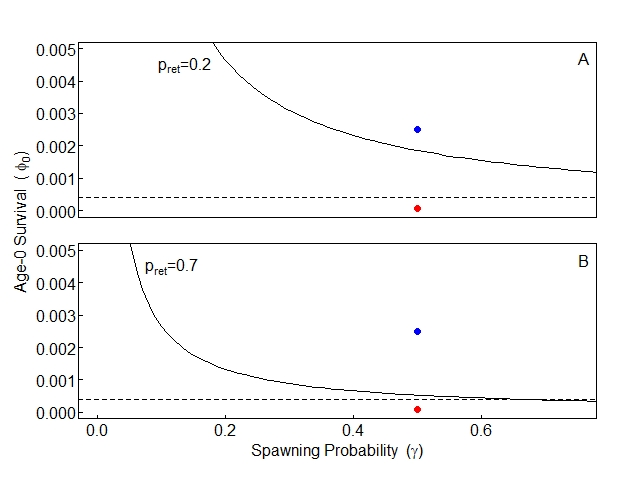
\includegraphics[width=6in]{NEPA_Fig_8-boundary-example}
\caption{Population growth-decline boundaries ($\lambda=1$) when retention probability is A) 20\% and B) 70\%.  All dots indicate a population whose reproductively-ready females spawn in the Missouri River 50\% of the time.  Red dots indicate a population where 75 out of every 1,000,000 eggs are expected to survive to age-1, and blue dots indicate a population where 25 out of every 10,000 eggs are expected to survive to age-1.  Red dots are in a region of decline (below and left of the curve), while blue dots are in a region of growth (above and to the right of the curve).  The dashed line indicates Pine et al.'s (2001) upper estimate of age-0 survival for gulf sturgeon, 0.0004.  Population growth at this survival level can occur but only at high spawning and retention probabilities.}
\label{boundaryEx}
\end{figure}

\begin{figure}[h]
\centering
\hspace*{-0.5in}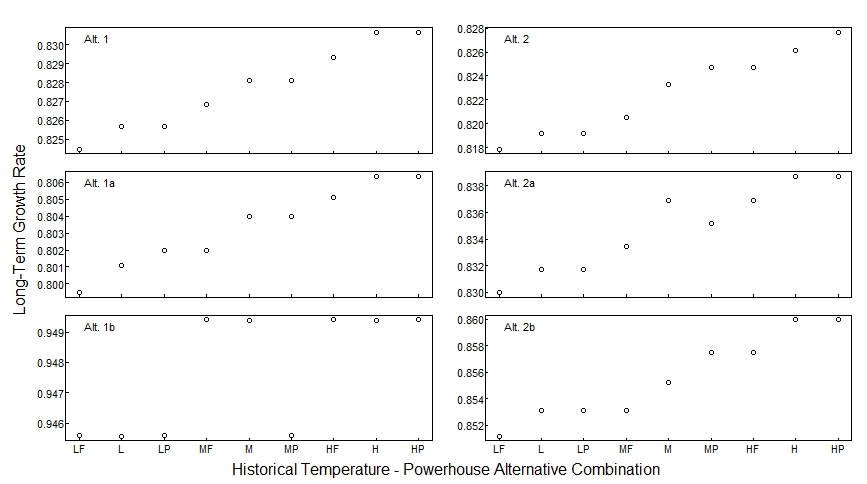
\includegraphics[width=7.5in]{NEPA_Fig_9-Year85-SA}
\caption{Long-term growth rate ($\lambda$) values for six Fort Peck flow scenarios under particular historical temperature and powerhouse operation combinations: LF--low temperature, full powerhouse operations; L--low temperature, standard powerhouse operations; LP--low temperature, peak time powerhouse operations, and similar for M--median temperature and H--high temperature.  \textit{Check:  Median temperatures were taken over the historical period of record (years), while low and high temperatures were estimated as the lower and upper 95\% confidence intervals.} Full powerhouse operations assume 14kcfs are run through the powerhouse 24 hours a day; standard powerhouse operations assume 14kcfs are run through the powerhouse for 12 hours a day with 7kcfs running through the powerhouse the remaining 12 hours; peak time powerhouse operations assume 7kcfs are run through the powerhouse except during peak times (\textit{times here}) when 14kcfs are run through.}
\label{SA85}
\end{figure}

\end{document}